% !TeX root = ..\protokoll.tex
\documentclass[../protokoll.tex]{subfiles}
\graphicspath{{\subfix{../images/}}}
\begin{document}
\section{Bestimmung des Durchmessers von Airy-Scheiben}
Für diesen Versuchsteil wird der Versuchsaufbau des vorhergegangenen Versuchs verwendet. Allerdings wird für diesen Versuch die bisher verwendete Linse durch eine Linse mit einer Brennweite $f = 300$ mm ersetzt. Die Ausrichtung erfolgt so, dass der Brennpunkt der Linse Mittig zum CCD-Sensor liegt. Zudem wird der Spalt aus dem Versuchsaufbau entfernt. Stattdessen werden in den Blendenbehälter, der vor der Linse montiert ist, nacheinander zwei Lochblenden unterschiedlichen Durchmessers eingesetzt. Diese werden durch den Laser beleuchtet, was eine Beleuchtung durch eine unendlich weit entfernte Punktlichtquelle simuliert. Das jeweilige Beugungsbild wird aufgenommen und anschließend der Profilschnitt durch das Zentrum den Beugungsbildes beobachtet. Ist der Abstand der ersten Minima links und rechts maximal, geht der Profilschnitt durchs Zentrum des Beugungsbildes. Die Daten werden auch für diesen Versuch in einer Textdatei gespeichert und können durch anschließenden Import zu Origin grafisch dargestellt werden. Anhand der gewonnenen Werte kann der Durchmesser $d$ der AIRY-Scheibe ermittelt werden. Der ermittelte Durchmesser $d$ wird danach mit den theoretischen Werten verglichen.

\subsection{Auswertung}
Für beide Lochblenden wird das Beugungsbild in der Brennebene der Linse aufgenommen, zu sehen in \cref{fig:v2-beugung-1,fig:v2-beugung-2}, sowie ein Profilschnitt durch das Zentrum des Beugungsbildes ermittelt den die \cref{fig:v2-schnitt-1,fig:v2-schnitt-2} zeigen.

\begin{figure}[H]
    \centering
    \begin{subfigure}[t]{0.24\textwidth}
        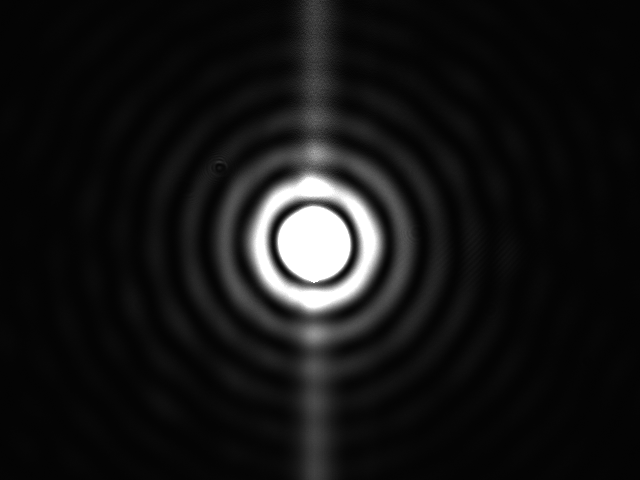
\includegraphics[width=\textwidth]{2023-05-15 - V5 - FRAUNHOFER- und FRESNEL-Beugung, Interferenz/images/v2/1mm.png}
        \caption{Beugungsbild der Lochblende mit dem Durchmesser 1,0 mm}
        \label{fig:v2-beugung-1}
    \end{subfigure}
    \hfill
    \begin{subfigure}[t]{0.24\textwidth}
        \includegraphics[width=\textwidth]{2023-05-15 - V5 - FRAUNHOFER- und FRESNEL-Beugung, Interferenz/images/v2/graph-1mm.png}
        \caption{Profilschnitt durch das Zentrum der Lochblende mit dem Durchmesser 1,0 mm}
        \label{fig:v2-schnitt-1}
    \end{subfigure}
    \hfill
    \begin{subfigure}[t]{0.24\textwidth}
        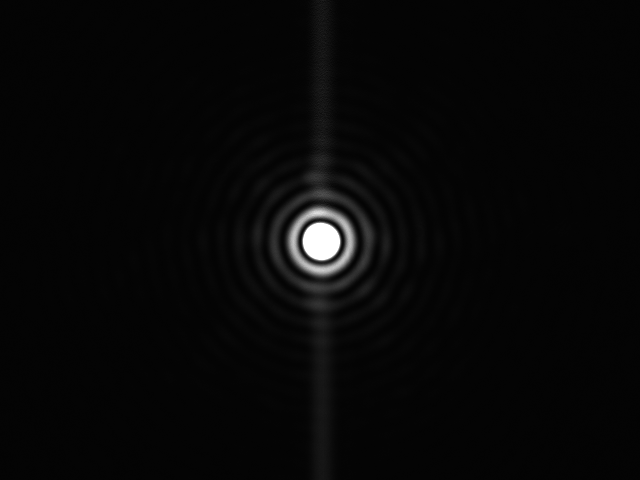
\includegraphics[width=\textwidth]{2023-05-15 - V5 - FRAUNHOFER- und FRESNEL-Beugung, Interferenz/images/v2/2mm.png}
        \caption{Beugungsbild der Lochblende mit dem Durchmesser 2,0 mm}
        \label{fig:v2-beugung-2}
    \end{subfigure}
    \hfill
    \begin{subfigure}[t]{0.24\textwidth}
        \includegraphics[width=\textwidth]{2023-05-15 - V5 - FRAUNHOFER- und FRESNEL-Beugung, Interferenz/images/v2/graph-2mm.png}
        \caption{Profilschnitt durch das Zentrum der Lochblende mit dem Durchmesser 2,0 mm}
        \label{fig:v2-schnitt-2}
    \end{subfigure}
    \caption{Aufgenommene Daten als Abbildungen und Graphen}
    \label{fig:v2}
\end{figure}

Theoretisch gilt gemäß \cref{fig:skizze-durchmesser} wenn eine kreisförmige Lochblende mit dem Durchmesser $D$ mit einer ebenen Lichtwelle $E$ der Wellenlänge $\lambda$ beleuchtet wird, dann ist beim entstehenden Beugungsmuster in der Ebene S (liegt parallel zur Ebene der Lochblende und ist von dieser unendlich weit entfernt) die Lichtintensität $I$ an einem Punkt P in S, der vom Ursprung von S die Entfernung $\rho$ und vom Mittelpunkt der Lochblende die Entfernung $R$ hat, gegeben durch:
\begin{equation}\label{eq:v2-1}
    I(P) = I_0 \left( \dfrac{
        2 J_1 \left( \dfrac{k D \rho}{2 R} \right)
    }{
        \dfrac{k D \rho}{2 R}
    } \right)^2
\end{equation}
wobei $I_0$ die Intensität im Ursprung von S und $J_1$ ist die \textsc{Bessel}-Funktion erster Ordnung un erster Art.

Mit
\begin{equation}\label{eq:v2-0}
    \sin \theta = \dfrac{\rho}{R}
\end{equation}
und der Abkürzung
\begin{equation}\label{eq:v2-0.5}
    q = k \dfrac{D}{2} \sin \theta = \dfrac{\pi D}{\lambda} \sin \theta
\end{equation}
bekommt \cref{eq:v2-1} die folgende vereinfachte Form
\begin{equation}
    I(q) = I_0 \left( \dfrac{2 J_1(q)}{q} \right)^2
\end{equation}
\begin{figure}[H]
    \centering
    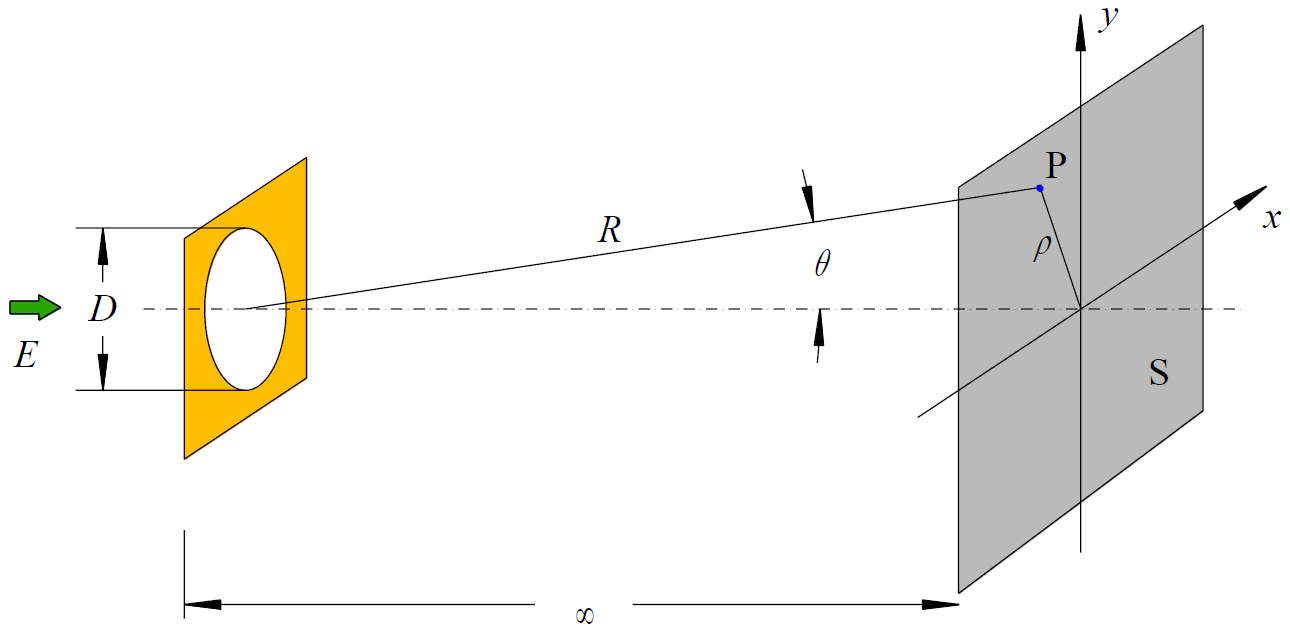
\includegraphics[width=0.6\textwidth]{2023-05-15 - V5 - FRAUNHOFER- und FRESNEL-Beugung, Interferenz/images/v2/skizze-v2.png}
    \caption{Skizze zur Beugung an einer kreisförmigen Blende vom Durchmesser $D$, entnommen aus \cite{script}}
    \label{fig:skizze-durchmesser}
\end{figure}

Der helle Kreis im Zentrum eines Beugungsbildes (vgl. \cref{fig:v2-beugung-1,fig:v2-beugung-2}) wird als \textsc{Airy}-Schreibe bezeichnet.
Der Radius dieser Scheibe entspricht dem Wert $q$, bei dem $I(q)$ nach \cref{eq:v2-1} die erste Nullstelle hat, also
\begin{equation}
    I(q_0) = I_0 \left( \dfrac{2 J_1(q_0)}{q_0} \right)^2 = 0 \to \qquad q_0 \approx 3,3817
\end{equation}

Wird nun zut Beobachtung eines Beugungsbildes eine Linse der Brennweite $f$ eingesetzt, so bezeichnet $\rho$ nun die radiale
Koordinate in der Brennebende der Linse. Somit wird aus \cref{eq:v2-0}:
\begin{equation}
    \sin \theta = \dfrac{\rho}{f}
\end{equation}

und aus Gleichung \cref{eq:v2-0.5}
\begin{equation}
    q = \dfrac{k D \rho}{2 f} = \dfrac{\pi D \rho}{\lambda f}
\end{equation}

Damit lässt dich der Radius $\rho_0$ der \textsc{Airy}-Schreibe folgendermaßen berechnen
\begin{equation}\label{eq:radius}
    \rho_0 = \dfrac{q_0}{\pi} \dfrac{\lambda f }{D} \approx 1,22 \dfrac{\lambda f}{D}
\end{equation}

Experimentell wird für $D = 1$ mm ein Durchmesser von \qty{0.42 \pm 0.0112}{\mm} (Pixelanzahl: 75 $\pm$ 2 mit 1 Pixel = \qty{5.6}{\mu\meter})
und für $D = 2$ mm ein Durchmesser von \qty{0.21 \pm 0.0056}{\mm} (Pixelanzahl: 37 $\pm$ 1 mit 1 Pixel = \qty{5.6}{\mu\meter}) für die \textsc{Airy}-Schreibe ermittelt.

Die theoretisch erwarteten Werte, die mit \cref{eq:radius} für den Radius der \textsc{Airy}-Scheibe
berechnet werden sind:

Für $D = 1$ mm: \quad $\rho = \qty{0.2316 \pm 0.002}{\mm}$ \\
Für $D = 2$ mm: \quad $\rho = \qty{0.1158 \pm 0.001}{\mm}$.

Diese Werte decken sich in etwa mit den reellen Werten. Die leichten Abweichungen können auf
nicht optimalst ausgerichtete Verscuhsaufbauten oder auf Ablesefehler der Pixel zurückgeführt
werden, da hier durch Unschärfe keine genauen Grenzwerte ablesbar sind.

\end{document}